\documentclass[11pt,a4paper]{article}

\usepackage[T1]{fontenc}
\usepackage[utf8]{inputenc}
\usepackage{lmodern}
\usepackage{microtype}
\usepackage[margin=22mm]{geometry}
\usepackage{amsmath,amssymb}
\usepackage{booktabs,tabularx,array}
\usepackage{enumitem}
\usepackage{xcolor}
\usepackage{tikz}
\usetikzlibrary{arrows.meta,positioning,shapes.geometric,fit}
\usepackage{hyperref}

\definecolor{accent}{HTML}{24557A}
\definecolor{lightblue}{HTML}{EEF4F8}
\definecolor{lightgray}{HTML}{F3F4F5}
\definecolor{darkgray}{HTML}{4A4A4A}

\hypersetup{
  colorlinks=true,
  linkcolor=accent,
  urlcolor=accent,
  pdftitle={Unified Mobile Sensing Fleet Simulation Framework}
}

\setcounter{secnumdepth}{2}
\setcounter{tocdepth}{2}
\setlength{\parindent}{0pt}
\setlength{\parskip}{0.45em}
\setlist{nosep,leftmargin=*}
\newcolumntype{Y}{>{\raggedright\arraybackslash}X}
\newcommand{\code}[1]{\texttt{\detokenize{#1}}}

\title{\textbf{Unified Mobile Sensing Fleet Simulation Framework}}
\author{}
\date{}

\begin{document}

\maketitle
\vspace{-3.5em}

\section{Framework Overview}

The user workflow is:

\begin{center}
\textbf{Environment} $\longrightarrow$ \textbf{Fleet Configuration}
$\longrightarrow$ \textbf{Simulation} $\longrightarrow$ \textbf{Portfolio Analysis}
\end{center}

\begin{itemize}
  \item \textbf{Environment} defines the common spatial and temporal simulation setting.
  \item \textbf{Fleet Configuration} defines Demand, Supply, Dispatch, and Routing for each fleet.
  \item \textbf{Simulation} generates physical-vehicle operations, movement records, and vehicle-level sensing exposure across replications.
  \item \textbf{Portfolio Analysis} evaluates alternative physical-vehicle sensor portfolios using replication-level sensing outcomes.
\end{itemize}

The design objective is to represent heterogeneous fleet operations through configurable data sources, vehicle specifications, constraints, and policies while preserving one common simulation kernel. Fleet labels are therefore illustrative configurations, not separate simulator implementations.

\section{Unified Simulation Model}

The framework is a \textbf{task-driven, vehicle-agent-based, discrete-event simulation}. Physical vehicles are represented as vehicle agents, and all service requests or prescribed movements enter the kernel as Tasks.

\subsection{Task Representation}

The central execution contract is

\[
T_i=\left(r_i,[s_{i1},\ldots,s_{im_i}]\right),
\qquad
s_{ij}=\left(\ell_{ij},\bar t_{ij},\tau_{ij}\right),
\]

where $r_i$ is the Task release time, $\ell_{ij}$ is the TaskStep location, $\bar t_{ij}$ is an optional scheduled or target time, and $\tau_{ij}$ is an optional service time.

\begin{center}
\small
\begin{tabularx}{0.84\textwidth}{@{}lY@{}}
\toprule
\textbf{Service pattern} & \textbf{Task structure} \\
\midrule
Scheduled service & Ordered stop sequence with optional target times \\
Location service & One service location \\
OD service & Origin $\rightarrow$ destination \\
\bottomrule
\end{tabularx}
\end{center}

All demand sources are converted into this common Task representation before entering the simulation kernel. Fleet type is not hard-coded into Task execution.

\subsection{Vehicle Representation and Availability}

Supply creates the physical vehicle population. Each vehicle has a specification such as

\[
\mathrm{VehicleSpec}_v=
(\mathrm{id}_v,a_v,b_v,x_v^0,d_v,C_v,z_v),
\]

where $a_v$ and $b_v$ are individual start and end times, $x_v^0$ is the initial location, and depot $d_v$, capacity $C_v$, and service-area assignment $z_v$ are optional. Runtime Vehicle State records location, status, remaining capacity, and current Task.

Vehicle availability and Task availability are separate processes. A vehicle enters service at $a_v$ and leaves at $b_v$, independently of Task release times. Timetable data, observed fleet records, common shifts, or a supply model may generate the per-vehicle specifications; vehicles need not become active at the global simulation start.

\subsection{Event-Driven Simulation Kernel}

Simulation time advances directly to the next event time,

\[
t\leftarrow\min\{t_e:e\in\mathcal Q_{\mathrm{event}}\},
\]

rather than through fixed time steps. The first implementation focuses on events that can change system-level decisions: Task release, vehicle entry, vehicle availability, and vehicle exit. For a multi-step Task, the Task Executor may construct its movement and service timeline internally and schedule only the next relevant vehicle-availability event.

\begin{figure}[htbp]
\centering
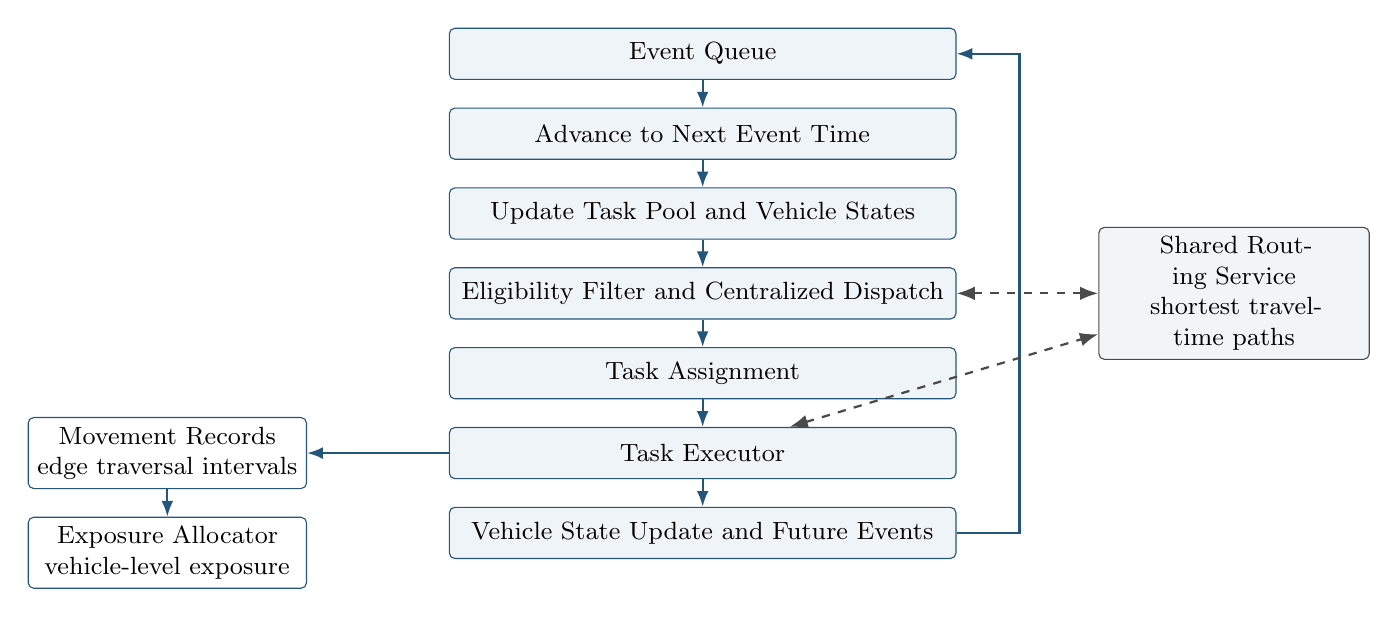
\begin{tikzpicture}[
  node distance=3.5mm,
  main/.style={rectangle,rounded corners=2pt,draw=accent,fill=lightblue,
               text width=6.2cm,minimum height=6.5mm,align=center,font=\small},
  service/.style={rectangle,rounded corners=2pt,draw=darkgray,fill=lightgray,
                  text width=3.2cm,minimum height=9mm,align=center,font=\small},
  output/.style={rectangle,rounded corners=2pt,draw=accent,fill=white,
                 text width=3.3cm,minimum height=8mm,align=center,font=\small},
  arrow/.style={-{Latex[length=2mm]},thick,draw=accent},
  query/.style={<->,>=Latex,dashed,thick,draw=darkgray}
]
  \node[main] (queue) {Event Queue};
  \node[main,below=of queue] (advance) {Advance to Next Event Time};
  \node[main,below=of advance] (state) {Update Task Pool and Vehicle States};
  \node[main,below=of state] (dispatch) {Eligibility Filter and Centralized Dispatch};
  \node[main,below=of dispatch] (assign) {Task Assignment};
  \node[main,below=of assign] (execute) {Task Executor};
  \node[main,below=of execute] (future) {Vehicle State Update and Future Events};

  \node[service,right=18mm of dispatch] (routing) {Shared Routing Service\\shortest travel-time paths};
  \node[output,left=18mm of execute] (movement) {Movement Records\\edge traversal intervals};
  \node[output,below=of movement] (exposure) {Exposure Allocator\\vehicle-level exposure};

  \draw[arrow] (queue) -- (advance);
  \draw[arrow] (advance) -- (state);
  \draw[arrow] (state) -- (dispatch);
  \draw[arrow] (dispatch) -- (assign);
  \draw[arrow] (assign) -- (execute);
  \draw[arrow] (execute) -- (future);
  \draw[arrow] (future.east) -- ++(0.8,0) |- (queue.east);
  \draw[query] (dispatch) -- (routing);
  \draw[query] (execute) -- (routing);
  \draw[arrow] (execute) -- (movement);
  \draw[arrow] (movement) -- (exposure);
\end{tikzpicture}
\caption{Common discrete-event simulation kernel. Routing is a shared service, not a single linear stage.}
\end{figure}

Simulation event time is distinct from sensing or reporting resolution. Movement intervals may later be allocated to 15-minute, hourly, or other reporting bins without changing the event-driven simulation clock.

\subsection{Dispatch and Eligibility}

At a dispatch event, the centralized Dispatch module observes the global waiting Task Pool and available Vehicle States. Before assignment, an eligibility filter constructs feasible vehicle--Task pairs:

\[
\mathrm{Eligible}(v,i)=1
\quad\text{if status, service-area, and capacity rules allow assignment.}
\]

Service area is a Supply-side operational constraint. Its input has two distinct parts: (i) service-area definitions, such as polygons or generated regions, and (ii) vehicle--area assignments. Internally, areas are represented by identifiers and spatial membership indices; Tasks are associated with an area through their relevant service-entry location. A shared depot may lie outside or serve several areas, so vehicle--area assignment is not inferred from initial location.

The first version exposes two policies:

\begin{itemize}
  \item \textbf{Predefined:} Task-to-vehicle assignments or sequences are determined before simulation.
  \item \textbf{Nearest Matching:} feasible pairs are matched centrally using shortest travel time from the shared Routing Service.
\end{itemize}

The same Nearest Matching policy naturally behaves as ``vehicle finds Task'' when a vehicle becomes available and as ``Task finds vehicle'' when a Task is released. These are state-dependent outcomes, not separate user-facing modes.

\subsection{Routing and Task Execution}

Routing is a shared Environment-level service. It provides travel-time queries to Dispatch and shortest-path movement legs to the Task Executor. The Task Executor connects the vehicle's current location and ordered TaskSteps, constructs edge-level movement and service intervals, updates the vehicle, and schedules the next relevant event.

Service Tasks and operational Tasks use the same executor. For example, when a vehicle has waiting service-area-eligible Tasks but insufficient remaining capacity for all of them, an operational policy creates a depot-return Task. The common executor routes the vehicle to the depot, resets capacity after replenishment, and makes the vehicle available again.

\section{Configurable Simulation Modules}

\begin{description}[style=nextline,font=\normalfont\bfseries]
  \item[Demand] Determines what service Tasks exist and when they become available. Observed records are standardized into Tasks. A demand model uses temporal patterns, spatial or OD distributions, optional service-time distributions, and optional quantities to generate Tasks. Generation may be completed before simulation or performed online.

  \item[Supply] Defines the physical vehicle population and produces per-vehicle specifications: individual operating times, initial locations, and optional depot, capacity, and service-area assignment. It also maintains runtime Vehicle States.

  \item[Dispatch] Applies eligibility constraints and either follows predefined assignments or performs centralized Nearest Matching. Optional operational policies may generate operational Tasks such as depot return.

  \item[Routing] Provides the shared shortest travel-time path service used by Dispatch and Task Execution. Alternative travel-time models can replace this service without changing the kernel.
\end{description}

\section{Input-to-Simulation Data Flow}

User data are transformed into a small set of runtime contracts before simulation begins.

\begin{center}
\scriptsize
\renewcommand{\arraystretch}{1.18}
\begin{tabularx}{\textwidth}{@{}p{1.65cm}Y Y Y@{}}
\toprule
\textbf{Component} & \textbf{Required data} & \textbf{Transformation} & \textbf{Used in simulation} \\
\midrule
Environment & Study area, road network, travel times, simulation horizon & Network graph, spatial index, Routing Service & Matching, routing, movement, event timing \\
Demand & Observed Task records or demand distributions/models & Standardized Tasks and Task-release events & Waiting Task Pool \\
Supply & Physical vehicle records or supply model; individual availability and initial locations; optional depot/capacity & Per-vehicle VehicleSpec and initial Vehicle State & Vehicle entry/exit, availability, operational state \\
Service area & Area polygons/generated regions and vehicle--area assignment & Area IDs, spatial membership, eligibility index & Eligibility filter before Dispatch \\
Dispatch & Policy and, if predefined, Task assignment & Dispatch policy state & Vehicle--Task assignment \\
Routing & Network and travel times & Shortest-path/travel-time service & Dispatch cost and Task movement \\
Sensing & Sensing grid, road--grid relationship, reporting bins & Edge--grid mapping and Exposure Allocator & Vehicle-level sensing exposure \\
\bottomrule
\end{tabularx}
\end{center}

\begin{figure}[htbp]
\centering
\begin{tikzpicture}[
  row distance=3mm,
  input/.style={rectangle,rounded corners=2pt,draw=darkgray,fill=lightgray,
                text width=4.0cm,minimum height=8mm,align=center,font=\scriptsize},
  transform/.style={rectangle,rounded corners=2pt,draw=accent,fill=lightblue,
                    text width=3.7cm,minimum height=8mm,align=center,font=\scriptsize},
  use/.style={rectangle,rounded corners=2pt,draw=accent,fill=white,
              text width=4.0cm,minimum height=8mm,align=center,font=\scriptsize},
  kernel/.style={rectangle,rounded corners=2pt,draw=accent,fill=accent!10,
                 text width=13.6cm,minimum height=10mm,align=center,font=\small},
  arrow/.style={-{Latex[length=1.8mm]},thick,draw=accent}
]
  \node[input] (i1) {Road network + travel times};
  \node[transform,right=7mm of i1] (t1) {Network graph + Routing Service};
  \node[use,right=7mm of t1] (u1) {Dispatch queries + Task movement};

  \node[input,below=3mm of i1] (i2) {Study area + sensing grid};
  \node[transform,right=7mm of i2] (t2) {Spatial index + edge--grid map};
  \node[use,right=7mm of t2] (u2) {Exposure allocation};

  \node[input,below=3mm of i2] (i3) {Demand records or distributions};
  \node[transform,right=7mm of i3] (t3) {Standardized Tasks + release events};
  \node[use,right=7mm of t3] (u3) {Waiting Task Pool};

  \node[input,below=3mm of i3] (i4) {Vehicle data or supply model};
  \node[transform,right=7mm of i4] (t4) {Vehicle specifications};
  \node[use,right=7mm of t4] (u4) {Vehicle entry + availability events};

  \node[input,below=3mm of i4] (i5) {Area definitions + vehicle--area mapping};
  \node[transform,right=7mm of i5] (t5) {Service-area membership index};
  \node[use,right=7mm of t5] (u5) {Eligibility filter};

  \foreach \a/\b in {i1/t1,i2/t2,i3/t3,i4/t4,i5/t5} {\draw[arrow] (\a) -- (\b);}
  \foreach \a/\b in {t1/u1,t2/u2,t3/u3,t4/u4,t5/u5} {\draw[arrow] (\a) -- (\b);}

  \node[kernel,below=7mm of t5] (runtime) {Task Pool + Vehicle States $\rightarrow$ Eligibility Filter $\rightarrow$ Centralized Dispatch $\rightarrow$ Assignment $\rightarrow$ Task Executor $\rightarrow$ Movement Records $\rightarrow$ Exposure Allocator};
  \node[fit=(u1)(u5),inner sep=1pt] (runtimeobjects) {};
  \draw[arrow] (runtimeobjects.south) |- (runtime.east);
\end{tikzpicture}
\caption{Transformation from user inputs to runtime simulation objects and sensing outputs.}
\end{figure}

\section{Sensing Exposure and Simulation Outputs}

The simulator need not generate second-by-second GPS points. Task execution produces shortest-path movement legs represented as road-edge traversal intervals. The Environment supplies an edge--grid spatial relationship, and the Exposure Allocator intersects movement intervals with spatial cells and configurable reporting time bins.

For replication $r$, the key sensing output is

\[
E^{(r)}_{v,g,t},
\]

the sensing exposure or sensing duration contributed by physical vehicle $v$ in grid cell $g$ and reporting interval $t$. This representation remains both vehicle-level and replication-level so that alternative sets of instrumented physical vehicles can be evaluated later.

The simulation produces three logical output categories:

\begin{enumerate}
  \item \textbf{Movement records:} vehicle path and movement intervals required for visualization and exposure allocation.
  \item \textbf{Operational records:} Task release, assignment and completion; Vehicle State changes; and service outcomes.
  \item \textbf{Vehicle-level sensing exposure:} $E^{(r)}_{v,g,t}$, with optional replication-level operational summaries.
\end{enumerate}

Simulation event time and reporting time bins are independent. Changing the sensing aggregation from 15 minutes to one hour changes exposure reporting, not event progression or fleet operations.

\section{Illustrative Fleet Configurations}

\begin{center}
\scriptsize
\renewcommand{\arraystretch}{1.15}
\begin{tabularx}{\textwidth}{@{}p{3.1cm}YYY@{}}
\toprule
 & \textbf{Scheduled service} & \textbf{Logistics} & \textbf{On-demand} \\
\midrule
Task structure & Stop sequence & Service location & Origin--destination \\
Demand generation & Usually pre-generated & Pre-generated or online & Observed or online-generated \\
Vehicle availability & Timetable/block-derived & Shift or vehicle-specific & Observed or generated \\
Initial location & First stop or depot & Depot or vehicle record & Spatial distribution or record \\
Service area & Optional & Optional, often operationally relevant & Optional \\
Capacity & Usually inactive & Optional & Optional \\
Baseline Dispatch & Predefined & Nearest Matching & Nearest Matching \\
\bottomrule
\end{tabularx}
\end{center}

These are illustrative compositions of the common modules, not hard-coded fleet types. Other combinations remain valid; for example, logistics demand may be online-generated, and scheduled Tasks may be dynamically assigned if the application requires it.

\section{Portfolio Interface}

Let $k$ index fleet configurations and let $x_{k,v}\in\{0,1\}$ indicate whether physical vehicle $v$ in fleet $k$ is instrumented. Replication $r$ retains vehicle-level exposure $E^{(r)}_{k,v,g,t}$. A candidate portfolio produces

\[
S^{(r)}_{g,t}(x)=\sum_k\sum_v x_{k,v}E^{(r)}_{k,v,g,t},
\qquad
U^{(r)}(x)=\Phi\!\left(S^{(r)}(x)\right),
\]

where $\Phi$ is the sensing-utility function. Portfolio Analysis evaluates $U^{(r)}(x)$ separately for every replication, then reports empirical means, standard deviations or variances, quantiles, and cost--utility--risk Pareto alternatives.

This order is essential when $\Phi$ is nonlinear:

\[
\frac{1}{R}\sum_{r=1}^{R}\Phi\!\left(S^{(r)}(x)\right)
\neq
\Phi\!\left(\frac{1}{R}\sum_{r=1}^{R}S^{(r)}(x)\right)
\quad\text{in general}.
\]

Replication-level vehicle exposure must therefore be preserved. Aggregated simulation summaries may support dashboards, but they do not replace the empirical replication outcomes required for nonlinear utility and uncertainty analysis.

\section{Extensibility}

The principal design rule is:

\begin{center}
\emph{New operational behaviors should modify policies or generate new Tasks rather than modify the simulation kernel.}
\end{center}

Rebalancing, charging, refueling, breaks, and depot return can be represented as operational Tasks; a new matching method is a Dispatch policy; a new demand process is a Demand source; and a new travel-time model replaces the Routing Service. All continue to use the same assignment, execution, state-update, and event-scheduling mechanism.

More complex future services such as ride pooling may require replacing a single next Task with a mutable vehicle plan. That extension is outside the first implementation and does not alter the present architectural boundary.

\end{document}
